% Conference paper, IEEEtran, A4, double-blind version.
% Generated from paper_content.py; the Word file is the same text.
\documentclass[conference,a4paper]{IEEEtran}
\IEEEoverridecommandlockouts
\usepackage{cite}
\usepackage{amsmath,amssymb,amsfonts}
\usepackage{graphicx}
\usepackage{array}
\usepackage{textcomp}
\usepackage[T1]{fontenc}
\usepackage[utf8]{inputenc}
\newlength{\tblw}
\def\BibTeX{{\rm B\kern-.05em{\sc i\kern-.025em b}\kern-.08emT\kern-.1667em\lower.7ex\hbox{E}\kern-.125emX}}
\begin{document}

\title{Reliability-Aware Clinical AI: A Cross-Modality Contract for Cardiovascular Decision Support}

\author{\IEEEauthorblockN{Anonymous Author(s)}
\IEEEauthorblockA{\textit{Affiliation withheld for double-blind review}}}

\maketitle

\begin{abstract}
Clinical machine learning is typically reported as a single accuracy figure, and the software around the model then treats every prediction as equally trustworthy. We contend that a deployed model must also indicate whether each prediction is reliable enough to act on, and we make that statement a first-class output. We describe a reliability contract: a modality-independent mapping from a prediction, its uncertainty, its input quality and its validity conditions onto five ordered decision states, actionable, caution, deferred, withheld and unavailable, so that a caller applies a single rule across every modality. Using four distinct cardiovascular cohorts, chest radiographs (MIMIC-CXR), 12-lead electrocardiograms (PTB-XL), echocardiogram video (EchoNet-Dynamic with CAMUS) and emergency-department triage records (MIMIC-IV-ED), we instantiate the contract and test each mechanism against a control that keeps the procedure and removes the signal. Three findings recur. Group-conditional deferral reduces the 6.68-point accuracy gap caused by acquisition metadata to -0.62, whereas uniform deferral of the same budget does not. A conformal guarantee that holds over the population fails inside 9 of 23 sex and age subgroups, which group-conditional calibration repairs in 22 of 23. Admitting a feature only once it existed at the decision time moves screening AUROC from 0.8763 to 0.9560 and exposes a label-circularity path we would otherwise have reported as accuracy. Under one common metric, the unsafe answer rate, abstention lowers unsafe answers in every component where coverage is measurable. Four ablations of our own design choices return three negative results.
\end{abstract}

\begin{IEEEkeywords}
abstention, clinical decision support, conformal prediction, covariate shift, data leakage, model reliability, selective prediction, subgroup validity, trustworthy AI
\end{IEEEkeywords}

\section{Introduction}
In a single day, a patient with chest pain who arrives at an emergency department produces four distinct kinds of data: a triage record of vital signs and a free-text complaint, an electrocardiogram within ten minutes \cite{ref1}, a chest radiograph taken early to rule out causes that are not cardiac \cite{ref2}, and an ultrasound scan of the beating heart. Each has become a machine-learning problem in its own right, and in each case the published result is typically one accuracy figure on one dataset.

A model that is about to sit behind an API is poorly described by one figure. It says nothing about the inputs on which the model is weakest, and in each of our four tasks those inputs are not rare corner cases but the sickest patients, an identifiable subgroup, the most severe grades, or a feature that did not exist when the decision was made. Table I names all four with the mechanism each one motivated. One is worth stating here, because it is why this paper exists: an audit of an earlier version of our own triage component found it reading its label out of a comorbidity column, and we rebuilt it from the raw tables.

Although the literature for each of these four issues is separate, the engineering response is the same each time: the model must expose when it should not be believed, in a form the calling code can branch on. We therefore treat reliability as the object of study rather than a property of any one network, and ask three questions. \textit{RQ1}, can reliability-aware mechanisms reduce clinically important failure modes without materially reducing predictive performance? \textit{RQ2}, can mechanisms as different as a group threshold, a conformal zone, a prediction interval and a disclosure horizon be represented by one contract? \textit{RQ3}, does reliability-aware abstention produce safer decisions than answering everything, or than deferring uniformly? The contributions are:

\begin{itemize}
\item a \textit{reliability contract}: five ordered decision states and a modality-independent rule for assigning them, so heterogeneous uncertainty vocabularies are reduced to a single field a caller can branch on without understanding how any component works;
\item a cross-modality evaluation of that contract on four distinct cardiovascular cohorts under a single measure, the unsafe answer rate, reported next to coverage so the cost of abstaining is priced rather than concealed;
\item controlled reliability experiments, one measured failure mode per modality, each with a control arm that keeps the procedure and removes the signal: acquisition shift, subgroup validity of a conformal guarantee, silent input corruption, open-set inputs, tail shrinkage under imbalance and temporal leakage;
\item four ablations of our own design choices, three of them negative results we report rather than bury, including a squeeze-and-excitation block that costs accuracy.
\end{itemize}

\section{Related Work}
Each modality has an established model family: convolutional classification over MIMIC-CXR \cite{ref3} with a ConvNeXt backbone \cite{ref4} and a BioBART decoder \cite{ref5}; one-dimensional residual networks over PTB-XL \cite{ref6}; video regression on EchoNet-Dynamic \cite{ref7} with an R(2+1)D backbone \cite{ref8}, with CAMUS \cite{ref9} as a smaller cohort richer in severe cases; and gradient-boosted trees \cite{ref10}, \cite{ref11} with post-hoc attribution \cite{ref12} over emergency-department tables \cite{ref13}. Saliency is typically Grad-CAM \cite{ref14}.

The reliability side has its own literature, which we use rather than reinvent. Subgroup performance gaps are established \cite{ref15}, equal opportunity \cite{ref16} is the standard metric, and fitting one threshold per group is the post-processing method proposed alongside it, so on this axis we claim the measurement and not the technique; the common alternative trains the offending factor out of the representation \cite{ref17}. A separate line lets the model abstain, from the reject option \cite{ref18} to conformal prediction, which converts a score into a decision carrying a finite-sample bound \cite{ref19}, \cite{ref20}, typically after calibration \cite{ref21}. Closest to our deferral finding is \cite{ref22}, which shows abstention can \textit{widen} group disparities; that is what our uniform-deferral control does, and the gap to the group-conditional version is our result. Ordinal targets employ rank-consistent heads \cite{ref23}, long tails deferred re-weighting \cite{ref24}, and leakage was formalised generally \cite{ref25}.

What we did not find was these ideas applied together, across more than one modality, with every mechanism tested against a null arm and the guarantee reported other than marginally.

\section{The Reliability Contract}
A component that cannot say when to disbelieve it forces the caller to guess, and every caller guesses differently. The contract makes that judgement an output. Each component keeps its own weights, uncertainty statistic and frozen decision rule; what it must additionally emit is a single field from five ordered states:

\begin{itemize}
\item \textit{actionable}, the component stands behind the result and the measured reliability we report for this kind of input applies;
\item \textit{caution}, the answer still stands, but a validity condition of that measurement does not hold here, so reliability is lower than headline;
\item \textit{deferred}, the component declines to commit and the case is referred;
\item \textit{withheld}, output was suppressed because a quality or verification gate rejected the input, so no probability is released at all;
\item \textit{unavailable}, the component could not run on this input.
\end{itemize}

The states are ordered from most to least usable, and that ordering is the whole interface: a caller applies one rule, do not act on a result that is not actionable, without knowing what a projection, a conformal zone or a disclosure horizon is. Assignment is a precedence cascade over four signals a component already computes: whether it ran, \textit{r}; whether the input passed its quality and verification gates, \textit{q}; an uncertainty statistic \textit{u} against a threshold \textit{tau} fitted on validation and frozen; and whether the validity conditions of the reported reliability hold here, \textit{v}. Numbering the states 0 to 4 in the order above, component \textit{m} returns

\begin{equation}
a_m \;=\; \max\!\bigl(0,\; \mathbf{1}[\neg v_m],\; 2\cdot\mathbf{1}[\neg q_m],\; 3\cdot\mathbf{1}[u_m < \tau_m],\; 4\cdot\mathbf{1}[\neg r_m]\bigr),
\end{equation}

so the least usable applicable state wins, and no component can be made to appear safer by an ordering accident. Over the set \textit{M}(\textit{x}) of components that saw patient \textit{x}, the assessment takes the same maximum,

\begin{equation}
a(x) \;=\; \max_{m \in \mathcal{M}(x)} a_m(x),
\end{equation}

which aggregates and deliberately does not fuse. Substituting a component alters only what fills \textit{u}, \textit{q} and \textit{v}; Section IV gives four such substitutions. States are returned as a normal response rather than an error status, since turning a safety mechanism into an error forces callers into retry loops around it.

\begin{figure}[!t]
\centering
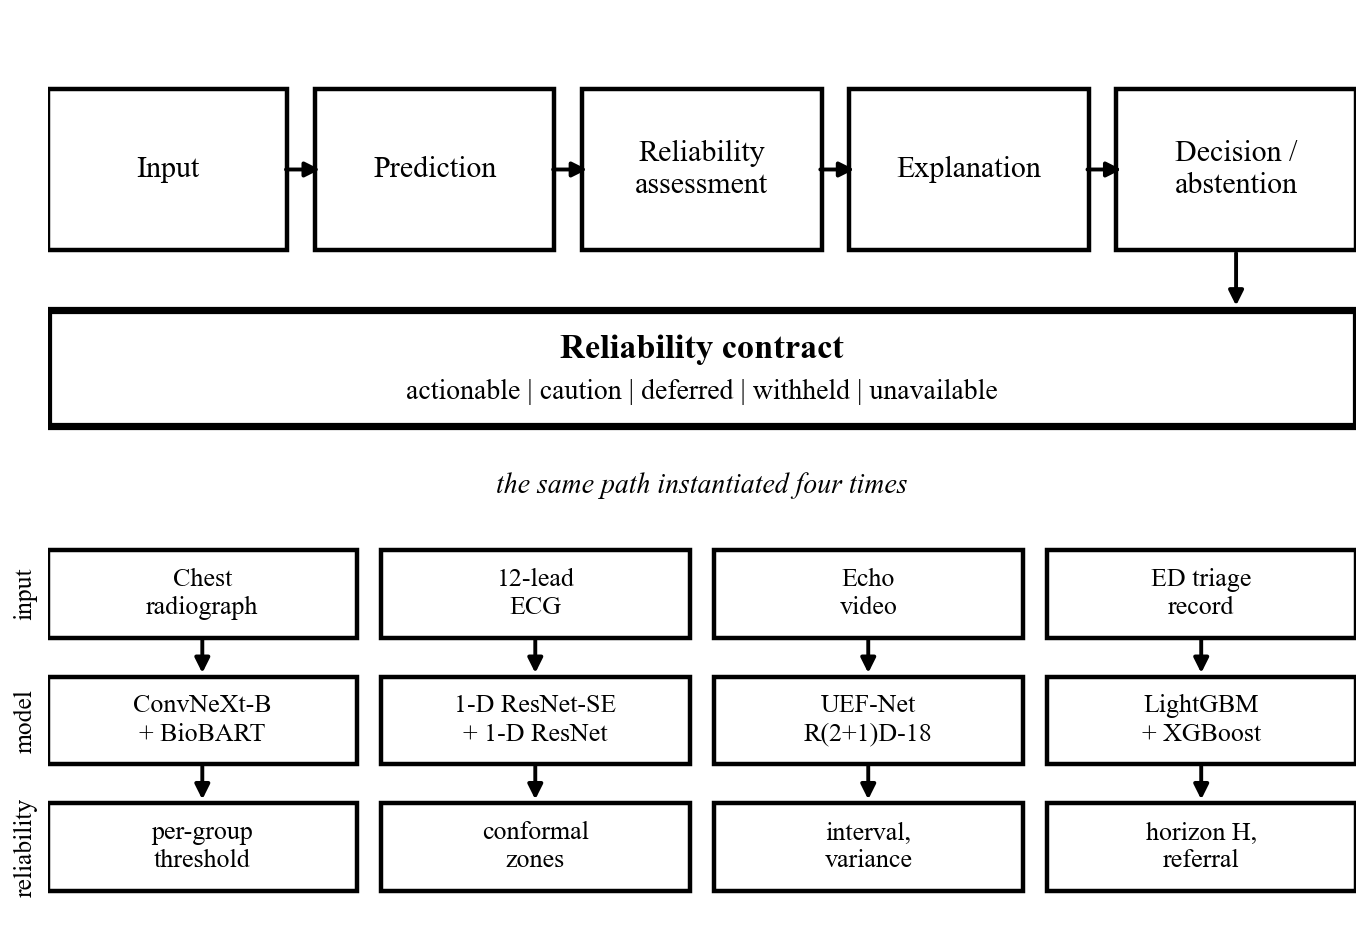
\includegraphics[width=\columnwidth]{figures/fig1_architecture.png}
\caption{The framework. One path runs left to right for every modality; the four cardiovascular components are instantiations of it, differing only in what fills the uncertainty, quality and validity slots.}
\label{fig:1}
\end{figure}

Aggregating rather than fusing is a limitation we measured, not a preference. Of the six cohort pairs only radiograph and triage are linkable, both deriving from MIMIC-IV and sharing 19,979 patients, 81.6 \% of the radiograph cohort; the other five share zero by construction. No patient carries all four studies, so this is a cross-modality framework evaluated on four distinct cohorts, not patient-level multimodal fusion; we train no fusion model and report no joint accuracy.

\section{Instantiating the Contract in Four Modalities}
Each subsection fills the same four slots for one modality: the quality gate \textit{q}, the uncertainty statistic \textit{u} and its frozen threshold, the validity condition \textit{v}, and the control arm the mechanism is tested against. The models are standard; the reliability machinery around them is the contribution.

\subsection{Covariate Shift from Acquisition Metadata}
A ConvNeXt-Base backbone \cite{ref4} produces eight sigmoid outputs from a 384 by 384 image; Grad-CAM \cite{ref14} is taken at the final feature block, and a BioBART decoder \cite{ref5} drafts report text we do not evaluate here. The network is not the interesting part. Each radiograph carries a metadata field \textit{g} in \{AP, PA\} recording how it was taken; the two groups are not the same distribution, so a single operating point for both is a modelling error. Following \cite{ref16}, we fit one per group on validation only,

\begin{equation}
\tau_g \;=\; \arg\max_{\tau}\; F_1\!\left(y_g,\; \mathbf{1}[\,p_g \ge \tau\,]\right),
\end{equation}

and apply the threshold belonging to the image's own group at inference. Ranking cannot change under (3), since AUROC is computed over the whole ordering and cutting each group at a different point reorders nothing. On top of it a selective rule refers the case when the prediction sits too close to the operating point,

\begin{equation}
m \;=\; \lvert p - \tau_g \rvert, \qquad \text{answer if } m \ge q_g, \ \text{else refer,}
\end{equation}

with \textit{q}(AP) and \textit{q}(PA) fitted on validation under one shared coverage budget, choosing the pair that minimises the absolute accuracy difference between groups, then frozen. At the deployed 85 \% coverage target they are 0.2247 and 0.0029, so the system is far more reluctant to commit on the weaker group. An image with no projection field falls back to the global threshold.

\subsection{A Guarantee, and Two Ways It Silently Stops Holding}
A quality gate checking shape, duration, dead leads, units, amplitude, noise and rhythm runs before the classifier, so a rejected recording never produces a probability. Accepted recordings are filtered, resampled and normalised per lead, then classified by a one-dimensional residual network with squeeze-and-excitation and attention pooling, followed by per-class temperature scaling \cite{ref21}. A triage layer converts each calibrated probability into one of three decisions under a training-conditional, or PAC, conformal bound \cite{ref19}. For a class with \textit{n} calibration positives, miss-rate budget \textit{alpha} and confidence \textit{delta}, the order statistic is

\begin{equation}
m^{*} \;=\; \max\left\{\,k \le n \;:\; F_{\mathrm{Beta}(k,\,n-k+1)}(\alpha) \ge 1-\delta \,\right\},
\end{equation}

since the coverage of the \textit{k}-th order statistic follows Beta(\textit{k}, \textit{n}-\textit{k}+1). The rule-out threshold is that order statistic among the positive calibration scores, the rule-in threshold its mirror over the negatives, and anything between is referred. A class with too few calibration positives is reported unattainable rather than approximated. Two models are served side by side, each with its own calibrator, and a class is ruled out only when both rule it out, so the merged miss rate is bounded by the tighter single-model bound at the expense of more referrals.

A bound like this depends on assumptions the input can break without appearing broken, so two checks withdraw the guarantee while leaving the prediction in place: one flags a swapped pair of limb electrodes from the polarity of one lead and the inversion of another, the other asks whether the rhythm is inside the label space at all, from an irregularity score thresholded on validation at a 5 \% false-positive budget. Either way the probabilities are still returned and only the bounded-miss-rate claim is withdrawn, which is the \textit{caution} state of (1) rather than \textit{withheld}.

\subsection{Ordinal Targets, Noisy Labels and a Long Tail}
An R(2+1)D-18 backbone \cite{ref8} takes 32-frame clips and four heads: regression, ordinal cumulative, auxiliary class and log-variance. The boundaries at 30, 40 and 55 are clinical conventions, and the label they cut is itself noisy, since two readers typically disagree by about 4 points. Treating it as exact throws information away, so the ordinal targets are soft,

\begin{equation}
s_k \;=\; 1 - \Phi\!\left(\frac{t_k - e}{\sigma}\right),
\end{equation}

where \textit{e} is the recorded value, \textit{t\_k} the \textit{k}-th boundary and \textit{sigma} = 4, so \textit{s\_k} is the probability that the true value lies above \textit{t\_k}. Unlike \cite{ref23}, rank consistency is structural rather than repaired after the fact: one severity score is compared against cut-points that increase by construction, because each gap is a softplus,

\begin{equation}
c_1 = a,\quad c_k = a + \sum_{j<k}\mathrm{softplus}(g_j),\quad z_k = f(x) - c_k,
\end{equation}

so the cumulative probabilities can never cross. Training uses a class-balanced sampler with deferred re-weighting \cite{ref24} from epoch 15. The second cohort is intensity-matched before being blended in, since a balanced sampler over-draws from it and would let the network use scanner brightness as a shortcut for severity. A regressor on a skewed target also shrinks predictions toward the mean, pushing the severe tail over the boundary at 30, so an expansion is fitted on validation and applied without changing the weights,

\begin{equation}
\hat{e}\,' \;=\; \bar{y} + \kappa\,(\hat{e}-\bar{x}),\qquad \kappa = \frac{\mathrm{sd}(y)}{\mathrm{sd}(\hat{e})}\ \text{clipped to } [1.0,\,1.7],
\end{equation}

after which the boundaries are re-optimised on validation lexicographically: worst-class recall, then balanced accuracy, then macro-F1.

\subsection{An Information-Availability Contract}
The rebuild of this component started from the leak described in Section I, so every feature declares an availability time \textit{a(f)} relative to arrival. At a disclosure horizon \textit{H} the admitted feature set is

\begin{equation}
\mathcal{F}_H \;=\; \{\, f \;:\; a(f) \le H \,\},
\end{equation}

and values are clipped to those recorded within \textit{H} hours. The same cohort, split and code are featurised at \textit{H} = 0, 6 and 24 hours, making accuracy against time a reported axis rather than an unstated assumption. Detection is a mean blend of a LightGBM and an XGBoost ensemble \cite{ref10}, \cite{ref11}; subtyping uses a single four-class model rather than a cascade, since a cascade compounds error. The operating point is a stated optimisation rather than a hand-tuned multiplier,

\begin{equation}
w^{*} = \arg\max_{w}\ \mathrm{macroF_1}\!\left(\arg\max_k w_k p_k\right)\ \ \text{s.t.}\ \ \min_k \mathrm{recall}_k(w) \ge \rho,
\end{equation}

with the recall floor \textit{rho} = 0.75, solved on validation over bootstrap resamples and frozen. A case whose top-two margin falls below the (1 - \textit{C}) quantile is referred to a clinician rather than subtyped. Results are reported on the intended-use population, visits with a cardiac complaint or an early electrocardiogram order, both observable at triage, so this is selection, not leakage. A separate head asks which wall of the heart the infarct involves.

\section{Experimental Setup}
Four public cohorts are used, every split patient-disjoint and quoted as train / validation / test. C1: MIMIC-CXR-JPG \cite{ref3}, 36,362 / 4,474 / 4,722 images, the test fold containing 2,891 bedside and 1,831 standing films, positive class enriched to 50.4 \%. C2: the official PTB-XL \cite{ref6} folds, 13,801 / 1,709 / 1,711 recordings, keeping only codes at full likelihood. C3: EchoNet-Dynamic \cite{ref7}, 7,465 / 1,288 / 1,277 studies, severity classes at 5.9 / 7.2 / 18.0 / 68.9 \%, plus 1,000 CAMUS \cite{ref9} clips in training only. C4: MIMIC-IV-ED \cite{ref13}, 142,111 / 30,453 / 30,452 stays grouped by patient, 2.65 \% positive. Each test split was evaluated once, and every decision rule in Section IV was fitted on validation and frozen before that split was opened. Metrics follow the task: AUROC, sensitivity, specificity and true-positive-rate disparity between acquisition groups \cite{ref16} for C1; per-class recall and NPV with the empirical miss rate against the promised bound for C2; mean absolute error, R$^{2}$ and minimum per-class recall for C3; AUROC, NPV and minimum per-class recall for C4. Coverage is quoted beside every selective number, since accuracy on the answered subset is not the accuracy of the system.

Differences are tested rather than eyeballed. Two rules scoring the same items are compared using McNemar's test \cite{ref26} in mid-\textit{p} form with Holm correction \cite{ref27} within each family; gaps and aggregate metrics use a paired bootstrap of 10,000 resamples on identical indices. Subgroup miss rates use exact binomial tests with Wilson intervals across all 23 cells; triage intervals are cluster bootstraps resampled by patient.

\section{Results}
Results come in four parts: headline detection accuracy per component, what each abstention rule buys against its control arm, four ablations of our own design choices, and a check that the deployed service reproduces the offline numbers.

\subsection{Detection Performance}
Detection accuracy is a precondition rather than the contribution, so we state it once. On its own test fold: C1 cardiomegaly AUROC 0.9189 at 92.3 \% sensitivity, n = 4,722; C2 macro accuracy 0.864 and recall 0.810, n = 1,711; C3 mean absolute error 3.979 ejection-fraction points and worst-class recall 0.723, n = 1,277; C4 screening AUROC 0.9560 at 99.41 \% negative predictive value and subtyping macro-F1 0.7448, n = 30,452. The rows are four tasks on four cohorts, not comparable with one another and none compared with a published benchmark, for the split reasons in Section VII.

\subsection{One Contract, Four Instantiations}
Table I answers RQ2 in one view: four failure modes with nothing in common, four mechanisms with nothing in common, and one contract state emitted by each. Every mechanism is stated against a control, so the improvement column is a difference rather than a level.

\begin{table}[!t]
\caption{The same contract instantiated four times. The action is the state the contract assigns when the mechanism fires; the improvement is measured against the control arm, never against a published benchmark.}
\label{tab:1}
\centering
\setlength{\tabcolsep}{3pt}
\setlength{\tblw}{\dimexpr\columnwidth-10\tabcolsep\relax}
\footnotesize
\begin{tabular}{|>{\raggedright\arraybackslash}p{0.080\tblw}|>{\raggedright\arraybackslash}p{0.200\tblw}|>{\raggedright\arraybackslash}p{0.320\tblw}|>{\raggedright\arraybackslash}p{0.180\tblw}|>{\raggedright\arraybackslash}p{0.220\tblw}|}
\hline
\textbf{Comp.} & \textbf{Failure mode} & \textbf{Mechanism and action} & \textbf{Control} & \textbf{Improvement} \\
\hline
C1 & Acquisition shift, AP vs PA & Per-group threshold; defer inside the margin (defer, caution) & Uniform deferral, same budget & Gap 6.68 to -0.62 points \\
\hline
C2 & Marginal bound invalid in subgroups & Group-conditional conformal zones; two-model consensus (withhold, refer) & Marginal conformal & Valid in 9 of 23 cells to 22 of 23 \\
\hline
C3 & Tail shrinkage at 11:1 imbalance & Ordinal head, variance expansion, boundary deferral (defer) & Full-coverage prediction & Severe recall 0.590 to 0.687 \\
\hline
C4 & Temporal leakage & Disclosure horizon H; constrained decision layer (refer) & Horizon sweep H = 0, 6, 24 h & AUROC 0.8763 to 0.9560 \\
\hline
\end{tabular}
\end{table}

\subsection{The Cost of Abstaining}
Accuracy on the answered subset flatters any system that abstains, so we report one measure that means the same thing in every modality. The \textit{unsafe answer rate} is the probability that the system both answers and is wrong, U = \textit{c} (1 - \textit{A}) for coverage \textit{c} and accuracy \textit{A} among answered cases; a component that never abstains has U equal to its error rate. Reported with coverage it prices abstention instead of concealing it. Fig. 2a gives all three components. The nuance is C1: uniform deferral reaches a marginally lower U than the group-conditional arm, 8.89 \% against 9.64 \% at the same budget, yet leaves the acquisition gap intact, which is exactly the trade the contract is meant to make visible. C3's 148 deferred studies are genuinely the hard ones, scoring 42.6 \% against 73.0 \% overall, and C4 buys its drop to 6.68 \% by deferring a third of subtyping decisions. Answering RQ3, abstention lowered the unsafe answer rate against the answer-everything arm in all three components, and in C1 only the group-conditional arm also removed the failure mode.

\begin{figure}[!t]
\centering
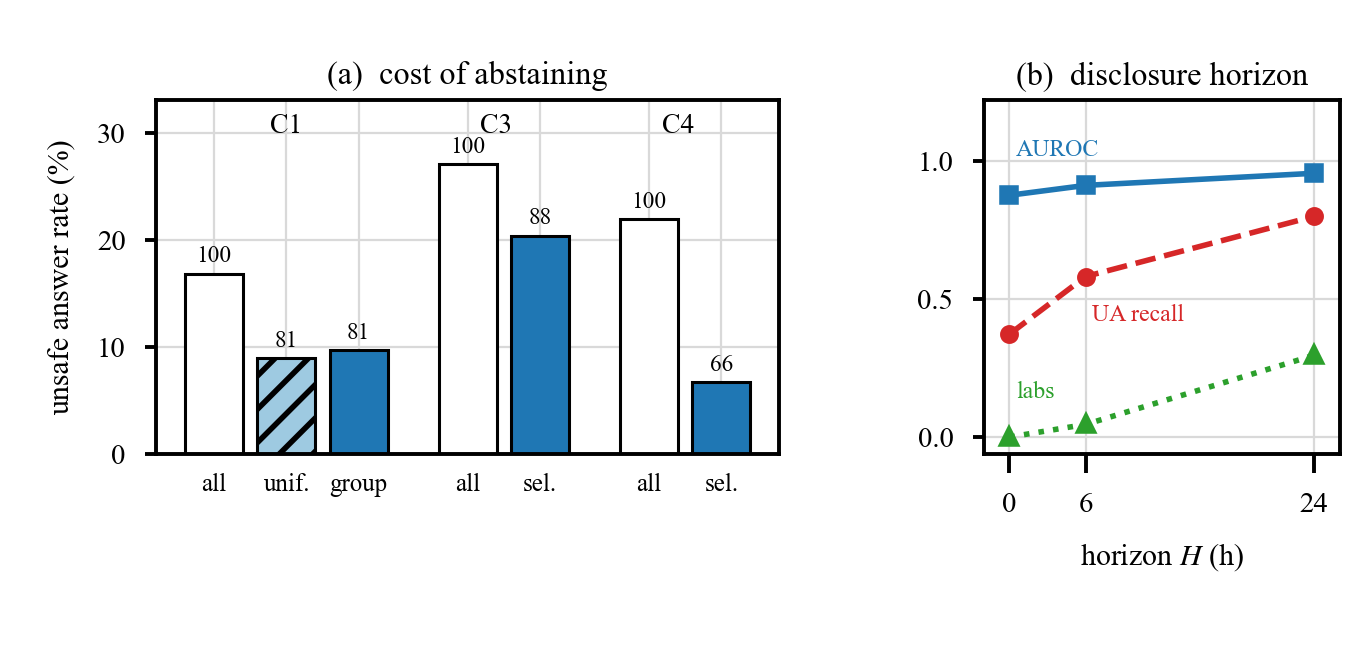
\includegraphics[width=\columnwidth]{figures/fig3_uar.png}
\caption{(a) Unsafe answer rate before and after abstention; the number above each bar is the coverage that arm retains, so the height is the risk and the label is its price. (b) Screening AUROC, unstable-angina recall and the share of attribution carried by laboratory features, against the disclosure horizon.}
\label{fig:2}
\end{figure}

\textit{Acquisition shift.} C1 scores AUROC 0.8224 on bedside images against 0.8864 on standing ones, a gap of 0.0639 [0.0491, 0.0790] in the same direction for all eight labels. Fitting the operating point per group cut the reported true-positive-rate disparity by 73.3 \% with an AUROC spread of exactly zero and no discernible accuracy cost (+0.02 points, McNemar mid-\textit{p} 0.885). We also reimplemented the representation-side alternative \cite{ref17} on our own data, backbone and split: it reached complete invariance, projection-detection AUC 0.5000, and still made the disparity 25.4 \% \textit{worse} at a cost of 0.0789 AUROC. Deferral behaves the same way (Fig. 2a): deferring uniformly leaves the gap at 6.28, the behaviour \cite{ref22} describes, while deferring per group at matched coverage closes it, a difference of 5.83 points with paired bootstrap \textit{p} = 0.0004.

\textit{Conditional validity.} Fitted marginally, the conformal bound held in only 14 of 23 class-by-subgroup cells, and two violations survive Holm correction: miss rates of 0.333 against a promised 0.10 under age 50, and 0.330 against 0.20 at age 70 and over. Refitting one threshold per subgroup \cite{ref20} restored the bound in 22 of 23, at the expense that every cell now needs its own positives: one cell with 42 cannot support a finite threshold and is reported unattainable.

\textit{Silent corruption and open-set inputs.} Simulating each of the three limb-electrode swaps on 200 test recordings, the corrupted signal passes the quality gate in 197 to 198 of them, because the recording is clean but wired wrongly; up to 87 \% of diagnoses change and 7 guarantees are voided. The physiology check detects 65.5 \% and 60.5 \% of two swaps at 4.5 \% false positives. Separately, 114 recordings carry a rhythm the label space cannot represent, and the irregularity gate withholds the bounded claim on 48.9 \% of them.

\textit{Shrinkage under imbalance.} On identical weights, the expansion in (8) lifted recall on the rarest class from 0.590 to 0.687, and seed averaging carried the worst class to 0.723. Selective prediction, which helped C1, failed here: at 88.4 \% coverage worst-class recall fell to 0.706 while overall accuracy rose. The uncertainty signal is sound, since accuracy on deferred studies is 0.426 against 0.770 on answered ones; the problem is geometric, in that one class occupies a 10-point interior band and abstention removes its members first.

\textit{Temporal leakage.} One comorbidity column equals 1 for every positive stay and reaches AUROC 0.9200 alone; adding it back to an otherwise safe feature set moves the screen from 0.9665 to 0.9889, which is how an apparently outstanding result gets manufactured. A random split places 5,804 patients on both sides and contaminates 7,627 test rows; the patient-grouped split shares none. Under the availability contract performance becomes a function of time (Fig. 2b), and recall on the hardest subtype moves 37.3 \%, 58.2 \%, 80.0 \% at \textit{H} = 0, 6, 24. At \textit{H} = 0 the laboratory channel carries exactly 0.0 \% of the attribution mass, rising to 4.6 \% and 29.6 \%; a leaking pipeline cannot produce that pattern.

\subsection{Turning the Same Standard on Our Own Designs}
The mechanisms above were tested against controls. So were four of our own design choices, and three came back negative. The sharpest is C2's architecture, which adds three things to a plain one-dimensional residual network. At three seeds each, compared by paired bootstrap on the untouched fold, they do not earn their 566 k parameters: the stem and attention pooling change nothing (\textit{p} = 0.741), and squeeze-and-excitation costs 0.0042 macro-AUROC (\textit{p} = 0.0040). Almost the whole loss sits on one class, +0.0147 AUROC without it, and there is a mechanism rather than a coincidence: that diagnosis is read from QRS amplitude, and squeeze-and-excitation recalibrates channels by learned importance, an operation on relative amplitude across leads.

C4's infarct-wall head is the second. With every feature it reaches AUROC 0.9074 on 104 test cases; removing three features parsed from the printed interpretation of the recording device costs 0.133 AUROC, and those three alone reach AUROC 0.841. This is not temporal leakage, since they exist at triage, but the person who assigned the diagnosis code read the same printout. Feature and label therefore share a source: the label is partly defined by an input the model is given, a circularity no timestamp check can detect. Widening the head beyond two territories was measured too, and a third class is recalled in 1 case of 12. C3's backbone was tested against the un-factorised alternative at three matched seeds and is worth keeping, though only on the classification metrics. Text generation exists in two components but is not evaluated here, and neither it nor the wall head is served.

Research and serving code drift apart, so the radiograph endpoint was also scored on 200 stratified real studies posted through the live HTTP path: served accuracy 0.790 [0.728, 0.841] at 14.0 \% deferred, and 0.766 on bedside images against 0.833 on standing ones. The covariate shift reappears on real inputs through the deployed path.

\section{Discussion, Threats to Validity and Limitations}
Answering RQ1 and RQ3 together: in these experiments the effective intervention was in the decision layer rather than the representation. Three attempts to close the acquisition gap by altering the model failed against a null arm, while a threshold and a deferral budget conditioned on the same variable worked, and the unsafe answer rate fell in every component where coverage is measurable. We do not conclude that clinical reliability is generally post-processing. We draw a narrower conclusion: on these four tasks, several reliability problems were addressed effectively by decision-layer controls that are inexpensive to fit and auditable, and conditioning each control on the variable that truly causes the failure mattered more than the strength of the control. RQ2 is answered by construction and tested through use: four mechanisms with nothing in common reduced to one five-state field without losing information, since the component-native payload is returned alongside it.

\textit{Threats to validity.} All four cohorts are retrospective and public, so distribution, labelling convention and case mix reflect the institutions that released them: MIMIC-CXR and MIMIC-IV-ED from one US hospital, PTB-XL from a German cohort of the 1990s, EchoNet-Dynamic from one US centre and CAMUS from one French centre. No result here transfers to another site without being re-measured. Every reliability threshold is fitted on validation and frozen, so it inherits that cohort's case mix; the coverage targets and the recall floor \textit{rho} = 0.75 are chosen by us, not derived from a clinical standard. There is no external validation, no prospective evaluation, no clinician-in-the-loop study and no patient outcome measured, so we can report that a decision was withheld but not whether withholding it benefited anyone. Without fully paired multimodal data, the aggregation rule of Section III is tested per component and not end to end.

\textit{Limitations.} The C1 split is custom, its positive class enriched to 50.4 \%, and 98.3 \% of its test images fall inside the official MIMIC-CXR training split; we therefore treat it as an internal operating point, make no comparison with published MIMIC-CXR benchmarks anywhere, and put a strict patient-level holdout first in further work. The same restriction applies to C2, which drops 21 \% of PTB-XL. Training variance is measured for C2 and C3 only, and subgroup coverage is partial: C1 has the acquisition field, C2 sex and three age bands, C3 none, C4 has them but no breakdown yet. The electrode audit rests on 200 recordings and the infarct-wall head on 104 test cases. C3's worst-class recall improved but fell short of the 0.75 target we set, on test and on validation. Grad-CAM is used as a sanity check rather than proof of localisation, its repeatability on chest radiographs assessed at a structural similarity of 0.12 \cite{ref28}, so we make no explainability claim beyond that. This is a retrospective research prototype, not a clinically validated system and not a medical device.

\section{Conclusion}
A deployed clinical model should not only produce a prediction; it should state whether that prediction is reliable enough to act on. We made that statement a first-class output through a reliability contract, five ordered states assigned by a precedence rule over a component's own quality, uncertainty and validity signals, and instantiated it in four cardiovascular modalities that share no patients and no features. Conditioning abstention on the variable that actually causes the failure beat altering the model in every comparison we ran, and lowered the unsafe answer rate wherever coverage could be measured. The same standard applied to our own design choices returned three negative results out of four. What the contract buys is that a caller applies one rule everywhere. Next are external validation, a strict patient-level holdout for C1, and a paired study on the 19,979 patients our radiograph and triage cohorts share.

\begin{thebibliography}{00}
\bibitem{ref1} R. A. Byrne et al., ``2023 ESC guidelines for the management of acute coronary syndromes,'' Eur. Heart J., vol. 44, no. 38, pp. 3720--3826, 2023.
\bibitem{ref2} M. Gulati et al., ``2021 AHA/ACC/ASE/CHEST/SAEM/SCCT/SCMR guideline for the evaluation and diagnosis of chest pain,'' Circulation, vol. 144, no. 22, pp. e368--e454, 2021.
\bibitem{ref3} A. E. W. Johnson et al., ``MIMIC-CXR-JPG, a large publicly available database of labeled chest radiographs,'' arXiv:1901.07042, 2019.
\bibitem{ref4} Z. Liu, H. Mao, C.-Y. Wu, C. Feichtenhofer, T. Darrell, and S. Xie, ``A ConvNet for the 2020s,'' in Proc. IEEE/CVF Conf. Comput. Vis. Pattern Recognit. (CVPR), 2022, pp. 11976--11986.
\bibitem{ref5} H. Yuan, Z. Yuan, R. Gan, J. Zhang, Y. Xie, and S. Yu, ``BioBART: Pretraining and evaluation of a biomedical generative language model,'' in Proc. BioNLP Workshop, 2022, pp. 97--109.
\bibitem{ref6} P. Wagner et al., ``PTB-XL, a large publicly available electrocardiography dataset,'' Sci. Data, vol. 7, art. 154, 2020.
\bibitem{ref7} D. Ouyang et al., ``Video-based AI for beat-to-beat assessment of cardiac function,'' Nature, vol. 580, pp. 252--256, 2020.
\bibitem{ref8} D. Tran, H. Wang, L. Torresani, J. Ray, Y. LeCun, and M. Paluri, ``A closer look at spatiotemporal convolutions for action recognition,'' in Proc. IEEE/CVF Conf. Comput. Vis. Pattern Recognit. (CVPR), 2018, pp. 6450--6459.
\bibitem{ref9} S. Leclerc et al., ``Deep learning for segmentation using an open large-scale dataset in 2D echocardiography,'' IEEE Trans. Med. Imag., vol. 38, no. 9, pp. 2198--2210, 2019.
\bibitem{ref10} G. Ke et al., ``LightGBM: A highly efficient gradient boosting decision tree,'' in Proc. Adv. Neural Inf. Process. Syst. (NeurIPS), 2017, pp. 3146--3154.
\bibitem{ref11} T. Chen and C. Guestrin, ``XGBoost: A scalable tree boosting system,'' in Proc. 22nd ACM SIGKDD Int. Conf. Knowl. Discovery Data Mining, 2016, pp. 785--794.
\bibitem{ref12} S. M. Lundberg and S.-I. Lee, ``A unified approach to interpreting model predictions,'' in Proc. Adv. Neural Inf. Process. Syst. (NeurIPS), 2017, pp. 4765--4774.
\bibitem{ref13} A. E. W. Johnson et al., ``MIMIC-IV, a freely accessible electronic health record dataset,'' Sci. Data, vol. 10, art. 1, 2023.
\bibitem{ref14} R. R. Selvaraju, M. Cogswell, A. Das, R. Vedantam, D. Parikh, and D. Batra, ``Grad-CAM: Visual explanations from deep networks via gradient-based localization,'' in Proc. IEEE Int. Conf. Comput. Vis. (ICCV), 2017, pp. 618--626.
\bibitem{ref15} L. Seyyed-Kalantari, G. Liu, M. McDermott, I. Y. Chen, and M. Ghassemi, ``CheXclusion: Fairness gaps in deep chest X-ray classifiers,'' in Proc. Pacific Symp. Biocomputing (PSB), 2021, pp. 232--243.
\bibitem{ref16} M. Hardt, E. Price, and N. Srebro, ``Equality of opportunity in supervised learning,'' in Proc. Adv. Neural Inf. Process. Syst. (NIPS), 2016, pp. 3315--3323.
\bibitem{ref17} S. C. Pereira, J. Rocha, A. Gaudio, A. Smailagic, A. Campilho, and A. M. Mendon\c{c}a, ``Addressing chest radiograph projection bias in deep classification models,'' in Proc. Med. Imag. Deep Learn. (MIDL), PMLR, vol. 227, 2023, pp. 1199--1210.
\bibitem{ref18} C. K. Chow, ``On optimum recognition error and reject tradeoff,'' IEEE Trans. Inf. Theory, vol. 16, no. 1, pp. 41--46, 1970.
\bibitem{ref19} V. Vovk, ``Conditional validity of inductive conformal predictors,'' in Proc. Asian Conf. Mach. Learn. (ACML), PMLR, vol. 25, 2012, pp. 475--490.
\bibitem{ref20} V. Vovk, D. Lindsay, I. Nouretdinov, and A. Gammerman, ``Mondrian confidence machine,'' Tech. Rep., 2003.
\bibitem{ref21} C. Guo, G. Pleiss, Y. Sun, and K. Q. Weinberger, ``On calibration of modern neural networks,'' in Proc. Int. Conf. Mach. Learn. (ICML), 2017, pp. 1321--1330.
\bibitem{ref22} E. Jones, S. Sagawa, P. W. Koh, A. Kumar, and P. Liang, ``Selective classification can magnify disparities across groups,'' in Proc. Int. Conf. Learn. Represent. (ICLR), 2021.
\bibitem{ref23} W. Cao, V. Mirjalili, and S. Raschka, ``Rank consistent ordinal regression for neural networks with application to age estimation,'' Pattern Recognit. Lett., vol. 140, pp. 325--331, 2020.
\bibitem{ref24} K. Cao, C. Wei, A. Gaidon, N. Arechiga, and T. Ma, ``Learning imbalanced datasets with label-distribution-aware margin loss,'' in Proc. Adv. Neural Inf. Process. Syst. (NeurIPS), 2019, pp. 1567--1578.
\bibitem{ref25} S. Kaufman, S. Rosset, C. Perlich, and O. Stitelman, ``Leakage in data mining: Formulation, detection, and avoidance,'' ACM Trans. Knowl. Discovery Data, vol. 6, no. 4, art. 15, 2012.
\bibitem{ref26} Q. McNemar, ``Note on the sampling error of the difference between correlated proportions or percentages,'' Psychometrika, vol. 12, no. 2, pp. 153--157, 1947.
\bibitem{ref27} S. Holm, ``A simple sequentially rejective multiple test procedure,'' Scand. J. Statist., vol. 6, no. 2, pp. 65--70, 1979.
\bibitem{ref28} N. Arun et al., ``Assessing the trustworthiness of saliency maps for localizing abnormalities in medical imaging,'' Radiol. Artif. Intell., vol. 3, no. 6, art. e200267, 2021.
\end{thebibliography}

\end{document}
